\documentclass[12pt,a4paper]{article}
\usepackage{parskip}
\usepackage[utf8]{inputenc} 
\usepackage{csquotes}
\usepackage{graphicx}
\usepackage[margin=2.54cm]{geometry}
\usepackage{fancyhdr}
\usepackage[spanish]{babel}
\usepackage[backend=biber,style=apa]{biblatex}
\DeclareLanguageMapping{spanish}{spanish-apa}
\addbibresource{bibliografia.bib}
\usepackage{microtype}
\usepackage[svgnames]{xcolor}
\usepackage{framed}
\definecolor{shadecolor}{named}{LightGray}
\pagestyle{fancy}
\fancyhf{}
\chead{Transtornos de la personalidad}
\rhead{Mateo Ardanaz}
\lhead{Universidad Católica}
\rfoot{\thepage}

\raggedright

\begin{document}

\section{El estudio cientifico de la personalidad}

En el lenguaje cotidiano se suele utilizar la palabra \textit{\enquote{personalidad}} como sinonimo de individuo o persona, sus cualidades y sus defectos. 

El estudio cientifico de la personalidad, es uno de los ambitos pioneros en investigacion de la psicologia. En terminos generales, los psicologos entienden l apersonalidad como el \textbf{conjunto de caractersiticas o rasgos que mejor describen o identifican el modo de ser y comportarse \textit{habitualmente} de un individuo}, de tal modo que podemos predecir con bastante exactitud su funcionamiento en otros contextos, actividades o situaciones vitales diferentes. 

Los psicologos no usan referencias evaluativas sobre los diferentes rasgos, es decir, no asumen que existan \textbf{rasgos positivos o negativos} \textit{per se}.

Tampoco se suelen concebir los rasgos en terminos de todo o nada (presencia vs ausencia), sino mas bien los caracterizamos en terminos de \textbf{dimensionales o continuos}. De esta manera un individuo puede manifestar mayores o menores niveles de introversion, agresividad, perfeccionismo, etc, dependiendo de la situacion en la que se encuentre. 

De este modo entonces la personalidad seria una \textbf{suma de propiedades y caracteristicas psicologicas} de distinos ordenes (emocionales, afectivas, cognitivas, comportamentales, sociales, etc), que caracterizan el modo de ser propio de un individuo y que lo identifican como tal, a traves del tiempo y de las diferentes situaciones y roles que desempeñe.

Esta propiedad se complejiza con el tiempo, ya que se haya en \textbf{cambio y crecimiento continuo}.

\subsection{Transtornos de personalidad o personalidades trasntornadas?: algunas precisiones y conceptos basicos}

El concepto de \textbf{transtorno psicologico o transtorno mental} hace referencia a una alteracion trasitoria de uno o mas aspectos del funcionamiento habitual de una persona, que tiene consecuencias negativas en diversos ambitos:

\begin{itemize}
	\item Su vida cotidiana.
	\item Su crecimiento y desarrollo individual.
	\item Su estado de animo.
	\item Sus relaciones personales. 
	\item Su comportamiento
\end{itemize}

En resumen, en todo lo que tiene que ver con la capacidad de \textbf{adaptabilidad} del sujeto. 

Estos cambios al ser egodistonicos\footnote{en contra del ego} provocan un gran sufrimiento personal, cosa que termina impregnando muchos aspectos de la experiencia personal de la persona. 

Los trasntornos mentales interfieren con el desarrollo de la persona, ya que dejan con bajo funcionamiento varias funciones-capacidades de la persona, por lo cual no pueden funcionar para la \textit{\enquote{mision}} que fueron diseñadas. 

Por otro lado los \textbf{transtornos de la personalidad} (TP) se caracterizan por:

\begin{itemize}
	\item Su aparicion temprana.
	\item Su estabilidad.
	\item Su resistencia al cambio
\end{itemize}

Esto se debe claramente a que uno de los aspectos fundamentales de la personalidad es que esta permanece \textbf{relativamente estable} a lo largo de toda la vida. Y esto se aplica tanto a personalidades normales, como a las trasntornadas. 

Cuando hablamos de TP hablamos que el modo de ser \textbf{habitual} del individuo es \textit{\enquote{enfermizo}}, patologico, anormal o disfuncional, ya sea porque:

\begin{itemize}
	\item No es el modo de ser mas frecuente de las personas de su entorno.
	\item No se ajusta a lo que cabria esperar de el (teniendo en cuenta su contexto socio-cultural).
	\item Porque no le permite desarrollar sus capacidades potenciales de una forma positiva y adecuada. 
	\item Etc\ldots
\end{itemize}

Hay que tener en cuenta sin embargo que \textit{\enquote{lo patologico no depende de los socialmente aceptado}}. Muchas veces el ambiente donde esta la persona es patologico en si y el individuo no por no tener el comportamiento de sus pares comparte sus padencias, sino que todo lo contrario.

Como mencionamos anteriormente, la \textbf{estabilidad de la personalidad} no es una cuestion de todo o nado, sino que \textbf{fluctua a lo largo de un continuo de intensidad}. Podemos ser unos reverendos soretes, pero que depende las situaciones ambientales este \textit{\enquote{soretismo}} se mueva en ese continuo de intensidad, llegando muchas veces hasta a anularse. 

En los TP, por el contrario sucede que la persona tiene un rasgo (o un conjunto de estos) de manera \textbf{extrema}, de tal modo que \textbf{siempre, o en la mayoria de los casos} su comportamiento o su modo de expresar emociones, de relacionarse con los demas, es \textbf{la misma, independientemente de lo que requiera la situacion}. Esto vendria a ser, si queremos una \textbf{extrema estabilida}

En consecuencia en los TP el \textit{\enquote{repertorio}} de comportamientos es \textbf{limitado, reiterativo e inflexible}. 

El segundo problema que se nos presenta es la \textbf{inestabilidad extrema de las caracteristicas personales}. El modo de ser y el comportamiento de la persona es sumamente impredecible, \textbf{incluso para ella misma}. Esto provoca qeu llegar a desarrollar estrategias consistentes de abordaje para los problemas que se presenten resulte casi imposible. El sujeto tiene una dificultad importante a la hora de saber lo que desea y no logra diseñar modos de lograrlo. 

En definitiva entonces tanto la \textbf{extrema estabilidad} (que da lugar a rigidez e inflexibilidad) como la \textbf{inestabilidad maxima} (que conlleva imposibilidad de predecir) de las caracteristicas basicas de la personalidad, son dos elementos nucleares de los TP. 

Los TP son \textbf{egosintonicos}, es decir, la persona no suele aceptar o entender su mal funcionamiento como mal funcionamiento. Una persona paranoide por ejemplo va a pensar que es exactamente lo cuidadosa y atenta que tiene que ser frente a los peligros del mundo y que el resto de personas estan locas por exponerse como se exponen. El malestar en estos casos se da mas por el lado de la \textbf{no aceptacion por parte de los demas del modo de ser del individuo}; la persona queda notoriamente ailada y en principio esos son los elementos que llevan principalmente a la persona a una sesion de terapia por cuenta propia.

\subsection{Clasificacion de los trasntornos de la personalidad: la perspectiva categorial}

Estas clasificaciones parten de la idea de que los TP \textbf{difieren unos de otros sobre la base de los rasgos que presentan}, los cuales se califican simplemente por su presencia o ausencia. \footnote{no se si en esta clasificacion los TP estan separados al eje 1.}

Este tipo de categorizacion no tiene en cuenta el aspecto dinamico; si el rasgo esta a determinado grado.

El problema aca es que el \textbf{solapamiento} que se produce entre los distintos trasntornos es mas que notable, cosa que acaba complicando ampliamente la decision diagnostica. 

Otro problema es el \textbf{solapamiento} de rasgos que se produce entre los distintos trasntornos es mas que notable, cosa que acaba complicando ampliamente la decision diagnostica. 

Otra critica que se les hace es porque carajo tienen una categoria propia. Mucha gente piensa que deberian estar junto a los trasntornos del eje 1. La respuesta de esto, es que muchos de los trasntornos mentales tienen una contraparte de TP pero como mas sarpados (ej: transtorno obsesivo compuslsivo de la personalidad vs el transtorno obsesivo del eje). La respuesta al tratamiento suele ser en terminos generales mejor para el trasntorno del eje 1 que para su supuesto homologo TP.

\subsection{La clasificacion de la Asociacion Americana de Psiquiatria (DSM-IV)}

En este sistema diagnostico los TP se clasifican en el \textbf{eje 2}, junto al retraso mental. La necesidad de separarlos se basa en \textbf{acentuar la invariabilidad/estabilidad a lo largo del ciclo vital de los TP}. 

\begin{figure}[!h]
	\centering
	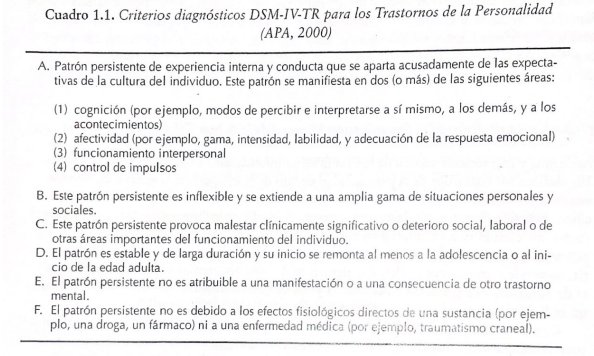
\includegraphics[width=0.7\linewidth]{hola.png}
	\label{fig:hola}
\end{figure}

El DSM-IV contempla 10 TP.

Tiene 3 grupos:

\begin{enumerate}
	\item Sujetos con personalidads franca y manifiestamente extrañas (paranoide, esquizoide y esquizotipico).
	\item Sujetos con inestabilidad emocional extrema y dificultas para controlar impulsos (antisocial, limite, histrionico y narcisista).
	\item Sujetos con ansiedad y/o miedo exagerados, motivados por un terror a perder el control en sentido generico  (por evitacion, por dependencia y obsesivo compulsivo).
\end{enumerate}

\subsection{La clasificacion de la Organizacion Mundial de la Salud (OMS)}

Esta clasificacion separa a los TP dentro de la categoria mas general llamada \textbf{transtornos de la personalidad y del comportamiento adulto}. 

Bajo esta etiqueta, ademas de los TP, se incluyen otros transtornos (habitos y control de impulsos, relacionados con el comportamiento y actividad sexuales). 

Se especifica que estos solo son \textbf{diagnosticables en adultos}. 

En este caso la clasificacion se hace en \textbf{5 grupos}. 

\subsubsection{Grupo 1: transtornos especificos de la personalidad}

Estos transtornos afectan las diversas facetas de personalidad del sujeto y las tendencias comportamentales del mismo. Estos trasntornos suelen aparecer durante la infancia o adolescencia y perduran durante toda la vida.

\begin{figure}[htpb]
	\centering
	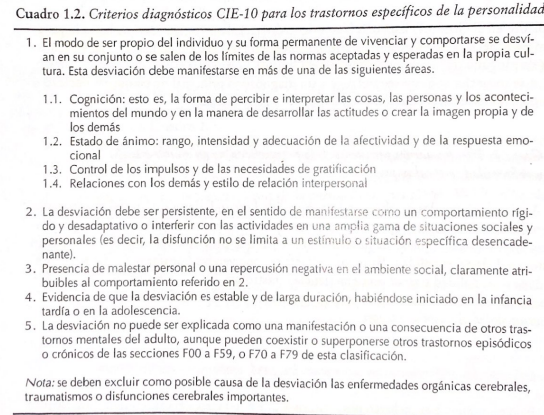
\includegraphics[width=0.7\linewidth]{hola1.png}
	\label{fig:hola1}
\end{figure}

Se recogen 8 transtornos de la personalidad:

\begin{enumerate}
	\item Paranoide.
	\item Esquizoide.
	\item Disocial.
	\item De inestabilidad emocional.
	\item Histrionico.
	\item Anancasico\footnote{ni idea que es esto}.
	\item Ansioso.
	\item Dependiente.
\end{enumerate}

El diagnostico de \textbf{transtorno de la personalidad no identificado} se reserva para aquellos transtornos que no satisfacen con claridad los criterios diagnosticos de ninguno de los contemplados anteriormente. 

\subsubsection{Grupo 2: transtornos mixtos y otros transtornos de la personalidad}

En esta categoria estan las anomalias de la personalidad que no tienen la sintomatologia concreta que destaca a los criterios diagnosticos del grupo 1.  

\subsubsection{Grupo 3: transformacion persistente de la personalidad no atribuible a lesion o enfermedad cerebral importante}

Aca estan los cambios de personalidad secundarios a \textbf{catastrofes o a exposiciones prologadas a factores estresantes intensos} o haber padecido enfermedades psiquiatricas importantes, y se manifiestan en sujetos que previamente no tenian ningun tipo de transtorno de la personalidad. 

\begin{itemize}
	\item Una experiencia catastrofica.
	\item Una enfermedad psiquiatrica.
\end{itemize}

\subsubsection{Grupo 4: otros transtornos de la personalidad y del comportamiento del adulto}

Aca tenemos a transtornos que refieren a la exageracion, fingimiento o prolongacion inadecuada en el tiempo de quejas somaticas, que en su inicio pueden ahber tenido una base real, o tambien pueden haber sido provocadas por el mismo sujeto a traves de autolesiones. En ambos casos la finalidad de los sintomas es \textbf{la obtencion de alguna ganancia secundaria de naturaleza consciente o intencionada}. 

\subsubsection{Grupo 5: transtornos de la personalidad y del comportamiento del adulto no especificados}

Esta categoria es basicametne el ultimo recurso. En estos casos la \textbf{carencia de informacion} no nos permite realizar un diagnostico concreto, sin embargo, hay una clara conviccion de que el paciente padece un trasntorno que afecta su personalidad. 

\subsection{Epidemiologia de los transtornos de la personalidad}

Se explica que los datos disponibles sobre la prevalencia de los TP son dispares y, en muchos casos, contradictorios y poco fiables. 

Dentro de todo se estima que la frecuencia de estos trasntornos en la poblacion general es elevada ($6-13\%$), y esa tasa aumenta cuando salimos de la poblacion general y entramos a la poblacion que padece de algun tipo de transtorno mental (entre el $20-40\%$).

En la mayoria de los estudios tambien se puede ver \textbf{una pequeña predominancia en las mujeres} frente a los hombres. 

Se especifica que los transtornos limites son los mas prevalentes dentro de estas cifras, y se explica que esto puede darse, no tanto por una cantidad real, sino por lo claros que son sus criterios diagnosticos.

Se plantea que los TP son \textbf{tanto o mas prevalentes} que los sindromes clinicos del eje 1 en la poblacion general. 

\subsection{Modelo multiaxial del DSM-IV}

Un sistema multiaxial implica una \textbf{evaluacion} en varios ejes



\newpage
\printbibliography[title={Bibliografía}]

\end{document}
